\documentclass{article}
\usepackage{amsmath}
\usepackage{amsthm}
\usepackage{enumerate}
\usepackage[bookmarks=true]{hyperref}
\usepackage{bookmark}
\usepackage{graphicx}
\usepackage{xcolor}

\usepackage{amssymb,amsmath,amsthm,amsfonts}
\usepackage{mathrsfs}
\usepackage{dsfont}
\usepackage{enumerate}

%\newtheorem{mdef}{Definition}
%\newtheorem{theorem}{Theorem}
\newcommand{\eqsplit}[2]{
  \begin{equation}\label{#2}
    \begin{split}
      #1
    \end{split}
  \end{equation}}
\newcommand{\eqnsplit}[1]{
  \begin{eqnarray*}
    #1
  \end{eqnarray*}}
\newcommand{\tran}[1]{
  \tilde{#1}
}
\newcommand{\td}[2]{
  \frac{d #1}{d #2}
}
\newcommand{\pd}[2]{
  \frac{\partial #1}{\partial #2}
}
\newcommand{\ppd}[2]{
  \frac{\partial^2 #1}{\partial #2^2}
}
\newcommand{\pdd}[3]{
  \frac{\partial^2 #1}{\partial #2 \partial #3}
}
\newcommand{\otd}[1]{
  \frac{d}{d #1}
}
\newcommand{\opd}[1]{
  \frac{\partial}{\partial #1}
}
\newcommand{\oppd}[1]{
  \frac{\partial^2}{\partial #1^2}
}
\newcommand{\opdd}[2]{
  \frac{\partial^2}{\partial #1 \partial #2}
}
\newcommand{\ket}[1]{
  |#1\rangle
}
\newcommand{\bra}[1]{
  \langle#1|
}
\newcommand{\inn}[1]{
  \langle#1\rangle
}
\newcommand{\mean}[1]{
  \langle#1\rangle
}
\newcommand{\tr}{
  \text{tr}\,
}
\newcommand{\re}{
  \text{Re}\,
}
\newcommand\im{
  \text{Im}\,
}
\newcommand{\var}{
  \text{var}
}
\newcommand{\arcsinh}{
  \sinh^{-1}
}
\newcommand{\arccosh}{
  \cosh^{-1}
}
\newcommand{\erfc}{
  \text{erfc}
}
\newcommand{\E}{
  \mathbb{E}
}
\renewcommand{\P}{
  \mathbb{P}
}
\newcommand{\I}[1]{
  \mathbf{1}_{\{#1\}}
}
\newcommand{\1}[1]{
  \mathds{1}_{\{#1\}}
}
\newcommand{\diag}{
  \text{diag\,}
}
\newcommand{\M}{
  {\text{max}}
}
\newcommand{\m}{
  {\text{min}}
}
\newcommand{\ph}{
  {\text{arg}\,}
}
\newcommand\erf{
  \text{erf}
}
\renewcommand\vec[1]{
  \mathbf{#1}
}
\newcommand\mtx[1]{
  \mathbf{#1}
}
\newcommand\ed{
  \,{\buildrel d \over =}\,
}




%% \newtheorem{theorem}{Theorem}
%% \newtheorem{lemma}{Lemma}
%% \theoremstyle{remark}
%% \newtheorem{remark}{Remark}

\newif\ifcomplete

\completetrue

\title{GARCH models for S\&P 500 and DAX}
\author{Xie Xiaolei}
\date{\today}

\begin{document}
\maketitle

\ifcomplete
\section{Introduction}
We consider the model
\begin{eqnarray*}
V_n &=& A_n V_{n-1} + B_n\\
\end{eqnarray*}
Use the following notations
\begin{eqnarray*}
X_n &=& {
        A_n A_{n-1} \cdots A_1 \tilde V_0
        \over
        |A_n A_{n-1} \cdots A_1 \tilde V_0|
        } \\
S_n &=& \log |A_n \cdots A_1 \tilde V_0| \\
\xi_n &=& S_n - S_{n-1} = \log\frac{|A_n \cdots A_1 \tilde V_0|}{|A_{n-1}
  \cdots A_1 \tilde V_0|} \\
&=& \log\left| A_n \frac{A_{n-1} \cdots A_1 \tilde V_0}
    {|A_{n-1} \cdots A_1 \tilde V_0|} \right|\\
&=& \log |A_n X_{n-1}|
\end{eqnarray*}
The pair $(X_n, S_n)$ is a Markov additive process with transition
kernel $P$. Assume conditions (M) and (A) of Kesten \cite{Kesten1973}:
\begin{enumerate}
  \item $\P(A > 0) = 1$, $\P(B \geq 0) = 1$, $\P(B = 0) < 1$.
   
\item
  \begin{enumerate}
  \item The top Lyapunov exponent is negative, i.e.
    \begin{equation}
      \label{eq:neg_top_Lyapunov}
      \inf_{n \geq 1} \E \log \|A_n \cdots A_1\| < 0    
    \end{equation}
  \item $\exists \xi > 0$ such that $\lambda(\xi) = 1$, where
    $$
    \lambda(\xi) := \inf_{n \geq 1} (\E \|A_n \cdots A_1\|^\xi)^{1/n}
    $$
    \item $\exists \epsilon > 0$ such that $\E \|A\|^{(1 + \epsilon)\xi} <
      \infty$ and $\E |B|^{(1 + \epsilon)\xi} < \infty$.
  \end{enumerate}
  \item The additive subgroup of $\mathbb R$ generated by
    \[
    \{\log \rho(\pi): \pi = \prod_{i=1}^n A_i \text{for some n and
      iid. } A_i\}.
    \]
    is dense in $\mathbb R$. Here $\rho(\pi)$ denotes the largest
    singular value of $\pi$.
\end{enumerate}

\section{Consistency}\label{sec:consistency}
By the law of large numbers
\begin{eqnarray*}
  && \P(|V| > u) \\
  &=& \lim_{n \to \infty} {1 \over n} \sum_{i=0}^n \1{|V_i| > u}
\end{eqnarray*}
Define
\[
R_n := \inf\{0 \leq i \leq n: V_i \in \mathcal C\}
\]
and
\[
K_i := \inf\{k \geq 1: k > K_{i-1}, V_k \in \mathcal C, K_0 = 0\}
\]
Then one can write
\begin{eqnarray*}
  && \lim_{n \to \infty} {1 \over n} \sum_{i=1}^n \1{|V_i| > u} \\
  &=& \lim_{n \to \infty} {1 \over n} \left[
    \sum_{i=0}^{K_{R_n}-1} \1{|V_i| > u} + \sum_{i=K_{R_n}}^n \1{|V_i| > u}
\right]
\end{eqnarray*}
For the 2nd term, by a Borel-Cantelli argument, it maybe shown
\[
\lim_{n \to \infty} {1 \over n}\sum_{i=K_{R_n}}^n \1{|V_i| > u} = 0
\]
For the 1st term,
\begin{eqnarray*}
&& \lim_{n \to \infty} {1 \over n} \sum_{i=0}^{K_{R_n}-1} \1{|V_i| >
  u}  \\
&=& \lim_{n \to \infty} {R_n \over n} {1 \over R_n} \sum_{i=1}^{R_n}
\sum_{j=K_{i-1}}^{K_i-1}\1{|V_i| > u} \\
&=& \pi(\mathcal C) \E_\gamma N_u
\end{eqnarray*}
where the law of large numbers of Markov chains has been used to reach
the last line. In addition, it is assumed
\begin{eqnarray*}
  V_{K_i} &\sim& \gamma \; \forall i \geq 0 \\
  \gamma(E) &=& \pi(E)/\pi(\mathcal C)\; \forall E \in \mathcal
  B(\mathcal C)
\end{eqnarray*}
Define
\begin{eqnarray*}
  T_u &=& \inf\{n \geq 1: |V_n| > u\} \\
  \tau &\overset{d}{=}& K_i - K_{i-1} \\
  N_u &:=& \sum_{i=0}^{\tau-1} \1{|V_i| > u}  \\
\end{eqnarray*}
Then $\E_\gamma N_u$ may be evaluated as
\begin{eqnarray*}
  && \E_\gamma N_u \\
  &=& \E_\gamma N_u \1{T_u < \tau} \\
  &=& \int_{\mathds S^{d-1}} \int_{\mathds R} \cdots \int_{\mathds
    S^{d-1}} \int_{\mathds R} N_u \1{T_u < \tau} \times \\
  && \prod_{i=1}^{T_u} e^{-\xi(s_i - s_{i-1}) + \lambda(\xi)}
  {r(x_{i-1}; \xi) \over r(x_{i}; \xi)}P_\xi(x_{i-1}, dx_i \times ds_i) \times \\
  && \prod_{i=T_u+1}^{\tau-1} P(x_{i-1}, dx_i \times d s_i) \\
  &=& \E_{\mathcal D} \left[
    N_u \1{T_u < \tau} e^{-\xi S_{T_u}} {r(\tilde V_0; \xi)
      \over r(x_{T_u}; \xi)}
  \right]
\end{eqnarray*}
where
\[
P_\xi(x_{i-1}, dx_i \times ds_i) = e^{\xi(s_i - s_{i-1}) -
  \lambda(\xi)} {r(x_i; \xi) \over r(x_{i-1}; \xi)} P(x_{i-1}, dx_i
\times ds_i)
\]
is the $\xi$-shifted transition kernel of the {\it Markov Additive
  process} $(X_n, S_n)$. $\xi$ is chosen such that 
\[
\lambda(\xi) = \lim_{n \to \infty} \log \left(
\E \|A_n \cdots A_1\|^\xi
\right)^{1/n} = 0
\]
$\E_{\mathcal D}$ denotes expectation taken with respect to the dual
measure defined as
\[
P_{\mathcal D} (x_i, dx_{i+1} \times ds) = \left\{
  \begin{array}{ll}
    P_\xi (x_i, dx_{i+1} \times ds) & \text{ if } i < T_u \\
    P(x_i, dx_{i+1} \times ds) & \text{ if } i \geq T_u \\
  \end{array}
\right.
\]
Because the top Lyapunov exponent is negative, it follows from a lemma
in Kesten \cite{Kesten1973} that there is a $s > 0$ such that
$\lambda(s) < 0$.

Thus we have obtained a consistent estimator
$\pi(\mathcal C)\mathcal E_u$ for $\P(|V| > u)$:
\begin{eqnarray*}
\P(|V| > u) &=& \pi(\mathcal C) \E_{\mathcal D} \mathcal E_u \\
&=& \pi(\mathcal C) \E_{\mathcal D} \left[
  N_u \1{T_u < \tau} e^{-\xi S_{T_u}} {r(\tilde V_0; \xi)
    \over r(x_{T_u}; \xi)}
\right]
\end{eqnarray*}

\section{Efficiency}\label{sec:efficiency}
\begin{lemma}
  Let $\beta \in \mathbb R$ satisfy
  \begin{enumerate}
  \item
    \begin{equation}
      \label{eq:drift_cond1}
      \E \|A\|^\beta < \infty      
    \end{equation}
  \item 
    \begin{equation}
      \label{eq:drift_cond2}
    \inf_{\alpha > 0} {\E \|A\|^{\alpha + \beta}
      \over 
      \E \|A\|^{\beta}
    } < 1
    \end{equation}
  \end{enumerate}
  then $\forall \alpha > 0$ such that $\frac{\E\|A\|^{\beta +
      \alpha}}{\E\|A\|^\beta} < 1$ , we have
  \begin{equation}
    \label{eq:drift}
    \E_\beta \left[\left.
        |V_n|^\alpha r_\beta(|\tilde V_n|; \alpha) \I_{{\mathcal C}^\complement}(V_{n-1}) \right|
      \mathcal F_{n-1} \right] \leq |V_{n-1}|^\alpha r_\beta(|\tilde
    V_{n-1}|; \alpha) \I_{{\mathcal C}^\complement}(V_{n-1})
  \end{equation}
  where $r_\beta(\cdot; \alpha)$ is the unique right eigen function of the
  operator
  \[
  P_{\beta, \alpha} f(x) = \int |\mathbf a x|^\alpha f\left(
    {\mathbf a x \over |\mathbf a x|}
  \right) d\mu_A^\beta(\mathbf a)
  \]
  where the $\beta$-shifted measure $\mu_A^\beta$ satisfies
  \[
  d\mu_A^\beta(\mathbf a) = {\|\mathbf a\|^\beta d\mu_A(\mathbf a) \over \E\|A\|^\beta}
  \]
  The set $\mathcal C = [-M_\beta(\alpha),
  M_\beta(\alpha)]$. $M_\beta(\alpha)$ is chosen with respect to the
  values of $\alpha$ and $\beta$.
\end{lemma}

\begin{proof}
  Conditions \eqref{eq:drift_cond1} and \eqref{eq:drift_cond2} imply $\E_\beta
  \|A\|^\alpha < \infty$. Then, using the results of Buraczewski and
  Collamore et al \cite{BCDZ2014}, one may conclude that an eigen
  function $r_\beta(\cdot; \alpha)$ as well as an eigen measure
  $l_\beta(\cdot; \alpha)$ exists under the $\beta$-shifted
  measure. Thus, by defining the adjoint operator under  the shifted
  measure, the right eigen function $r_\beta(x; \alpha)$ can be represented as
  \[
  r_\beta(x; \alpha) = c \int_{S_+^{d-1}} \inn{x, y}^\alpha
  dl^*_{\beta}(y; \alpha)
  \]
Now, to prove \eqref{eq:drift}, consider
  \begin{eqnarray}
    && \E_\beta \left[ |V_n|^\alpha r_\beta(\tilde V_n; \alpha) | \mathcal F_{n-1} \right]
    \nonumber \\
    &=& \E_\beta\left[\int_{S_+^{d-1}} \inn{V_n, y}^\alpha dl^*_{\beta}(y; \alpha)|
      \mathcal F_{n-1} \right]
    \nonumber \\
    &=& \E_\beta\left[\int_{S_+^{d-1}} (\inn{A_n V_{n-1}, y} + \inn{B_n,
        y})^\alpha dl^*_{\beta}(y; \alpha) | \mathcal F_{n-1} \right]
    \label{eq:drift_proof_1}
  \end{eqnarray}
  \begin{enumerate}
  \item if $\alpha \leq 1$, by subadditivity we have
    \begin{eqnarray*}
      &&\E_\beta\left[\int_{S_+^{d-1}} (\inn{A_n V_{n-1}, y} + \inn{B_n,
          y})^\alpha dl^*_{\beta}(y; \alpha) | \mathcal F_{n-1} \right]\\
      &\leq& \E_\beta\left[\int_{S_+^{d-1}} \inn{A_n V_{n-1}, y}^\alpha
        dl^*_{\beta}(y; \alpha) | \mathcal F_{n-1} \right]
      + \E_\beta\left[\int_{S_+^{d-1}} \inn{B_n, y}^\alpha dl^*_{\beta}(y; \alpha) |
        \mathcal F_{n-1} \right] \\
      &=& \E_\beta\left[|V_{n-1}|^\alpha |A_n \tilde V_{n-1}|^\alpha\int_{S_+^{d-1}}
        \inn{ {A_n \tilde V_{n-1} \over |A_n \tilde V_{n-1}|}, y}^\alpha
        dl^*_{\beta}(y; \alpha) | \mathcal F_{n-1} \right]  + \E r_\beta(B_n; \alpha)\\
      &=& |V_{n-1}|^\alpha  \int |\mathbf a \tilde V_{n-1}|^\alpha
      r_\beta\left({\mathbf a \tilde V_{n-1} \over |\mathbf a \tilde V_{n-1}|}; \alpha\right)
      d\mu_A^\beta (\mathbf a) + \E r_\beta(B_n; \alpha) \\
      &=& |V_{n-1}|^\alpha (P_{\beta, \alpha} r_{\beta})(\tilde V_{n-1}; \alpha) +
      \E_\beta r_\beta(B_n; \alpha) \\
      &=& |V_{n-1}|^\alpha r_\beta(\tilde V_{n-1}; \alpha) \lambda_\beta(\alpha)
      \left\{
        1 + 
        {\E_\beta r_\beta(B_n; \alpha) \over |V_{n-1}|^\alpha \lambda_\beta(\alpha) r_\beta(\tilde V_{n-1}; \alpha)}
         \right\} \\
    \end{eqnarray*}
    When $V_{n-1} \in \mathcal C^\complement$, $|V_{n-1}| > M_\beta(\alpha)$.
    Moreover, $\E_\beta|B_n|^\alpha < \infty$ by assumption while
    $r_\beta(\tilde B_n; \alpha) < \infty$, $r_\beta(\tilde V_{n-1}; \alpha) < \infty$
    according to Buraczewski and Collamore \cite{BCDZ2014}. Thus
    \begin{eqnarray*}
      && \E_\beta \left[ \left.
          |V_n|^\alpha r_\beta(\tilde V_n; \alpha) \I_{\mathcal C^\complement}(V_{n-1})
        \right| \mathcal F_{n-1}
      \right] \\
      &\leq&
      |V_{n-1}|^\alpha r_\beta(\tilde V_{n-1}; \alpha) \lambda_\beta(\alpha)
      \left[
        1 + 
        {\E_\beta r_\beta(B_n; \alpha) \over M^\alpha \lambda_\beta(\alpha) r_\beta(\tilde V_{n-1}; \alpha)}
      \right]
      \I_{\mathcal C^\complement}(V_{n-1})
    \end{eqnarray*}
    Also note
    \begin{equation*}
      \lambda_\beta(\alpha) \leq \E_\beta \|A_1\|^\alpha = {
        \E \|A_1\|^{\alpha + \beta}
        \over
        \E \|A_1\|^{\beta}
      }
    \end{equation*}
    Hence by assumption \eqref{eq:drift_cond2}, $\lambda_\beta(\alpha)
    < 1$. Therefore, $M_\beta(\alpha)$ can be chosen sufficiently large so that
    \begin{eqnarray}
      \lambda_\beta(\alpha) \left[
        1 +  
        {\E_\beta r_\beta(B_n; \alpha) \over M_\beta(\alpha)^\alpha
          \lambda_\beta(\alpha) r_\beta(\tilde V_{n-1}; \alpha)}
        \right] &<& 1 \label{eq:cond_on_M}
    \end{eqnarray}
    From \eqref{eq:cond_on_M} it follows
    \begin{equation}
      \label{eq:C_set}
      M_\beta(\alpha) > \left\{
        \bar r_{\beta, \alpha}\E_\beta |B|^\alpha
          \over
          [1 - \lambda_\beta(\alpha)] \underline r_{\beta, \alpha}
        \right\}^{1/\alpha}
    \end{equation}
    where
    \begin{eqnarray*}
      \bar r_{\beta, \alpha} &=& \sup_{x \in \mathbb S^{d-1}}
      r_\beta(x; \alpha) \\
      \underline r_{\beta, \alpha} &=& \inf_{x \in \mathbb S^{d-1}}
      r_\beta(x; \alpha)
    \end{eqnarray*}
    Here we note $\E_\beta |B|^\alpha = \E |B|^\alpha$
    since the distribution of $B$ is left the same when
    changing to the shifted measure.

    \item If $\alpha > 1$, applying Minkowski's inequality to the RHS
      of \eqref{eq:drift_proof_1} and using similar arguments as in
      the $\alpha \leq 1$ case gives
      \begin{eqnarray*}
        && \E_\beta \left[ \left.
          |V_n|^\alpha r_\beta(\tilde V_{n}; \alpha)
          \I_{\mathcal C^\complement}(V_{n-1})
          \right| \mathcal F_{n-1}
        \right] \\
        &\leq&
        |V_{n-1}|^\alpha r_\beta(\tilde V_{n-1}; \alpha)
        \lambda_\beta(\alpha) \left\{
          1 + \left[
            {
              \E r_\beta(B; \alpha)
              \over
              M_\beta(\alpha)^\alpha
              r_\beta(\tilde V_{n-1}; \alpha)
              \lambda_\beta(\alpha)
            }
          \right]^{1/\alpha}
          \right\}^\alpha
          \I_{\mathcal C^\complement}(V_{n-1})
      \end{eqnarray*}
      and correspondingly
      \begin{equation*}
        M_\beta(\alpha) > \left[
          {
            \bar r_{\beta,\alpha} \E |B|^\alpha
            \over
            \underline r_{\beta, \alpha}
          }
        \right]^{1/\alpha} {
          1 \over
          1 - \lambda_\beta(\alpha)^{1/\alpha}
        }
      \end{equation*}
  \end{enumerate}    
\end{proof}

\begin{remark}
  Iterating \eqref{eq:drift} yields
  \[
  \E_\beta \left[
    |V_n|^\alpha r_\beta(|\tilde V_n|; \alpha)
    \prod_{i=1}^{n-1}\I_{{\mathcal C}^\complement}(V_i)\right]
  \leq \rho_\beta(\alpha)^{n-1} |V_1|^\alpha r_\beta(|\tilde V_1|; \alpha) \I_{{\mathcal C}^\complement}(V_1)
  \]
  Then it follows
  \[
  \E_\beta \left[
    |V_n|^\alpha r_\beta(|\tilde V_n|; \alpha) \prod_{i=1}^{n}\I_{{\mathcal C}^\complement}(V_i)\right]
  \leq \rho_\beta(\alpha)^{n-1} |V_1|^\alpha r_\beta(|\tilde V_1|; \alpha) \I_{{\mathcal C}^\complement}(V_1)
  \]
  But $\prod_{i=1}^{n}\I_{{\mathcal C}^\complement}(V_i)$ implies $\tau > n$, and in this
  case $|V_n| > M$, where
  \[
  M = \left[
    \E_\beta (|B|^\alpha r_\beta(\tilde B; \alpha)) 
    \over
    (1 - \lambda(\alpha)) r_\beta(\tilde v; \alpha)
  \right]^{1/\alpha}
  \]
  Hence
  \begin{eqnarray}
    \E_\beta \left[
      M^\alpha \inf_{|\tilde V_n|} r_\beta(|\tilde V_n|; \alpha) \1{\tau > n}\right]
    &\leq& \rho_\beta(\alpha)^{n-1} |V_1|^\alpha r_\beta(|\tilde V_1|;
    \alpha) \I_{{\mathcal C}^\complement}(V_1) \nonumber \\
    \P_\beta(\tau > n) &\leq& K \rho_\beta(\alpha)^{n-1} \\
    &=& K [b \lambda_{\beta}(\alpha)]^{n-1} \label{eq:ret_time}
  \end{eqnarray}
  for some constant $K$ and some $b > 1$.
\end{remark}

\begin{theorem}
  The estimator $\mathcal E_u$ has bounded relative error, i.e.
  \begin{equation*}
    \limsup_{u \to \infty} {\var(\mathcal E_u) \over [\P(|V| > u)]^2} < \infty
  \end{equation*}
\end{theorem}
\begin{proof}
  The assertion is equivalent to
  \[
  \limsup_{u \to \infty} {\E_{\mathcal D} \mathcal E_u^2 \over [\P(|V|
    > u)]^2} < \infty
  \]
  By Kesten's theorem \cite{Kesten1973}, $\P(|V| > u) \sim C
  u^{-\xi}$. Hence, to prove the assertion, one needs to check
  $\limsup_{u \to \infty} u^{2\xi}\E_{\mathcal D} \mathcal E_u^2 <
  \infty$, i.e.
  \[
  \limsup_{u \to \infty} \E_{\mathcal D}  \left[u^{2\xi}
    N_u^2 \1{T_u < \tau} e^{-2\xi S_{T_u}} {r^2(\tilde V_0; \xi)
      \over r^2(x_{T_u}; \xi)}\right] < \infty
 \]
 Using the fact $|V_{T_u}| > u$, and that $r(\cdot; \xi)$ is bounded
 from above and below, it suffices to show
 \begin{eqnarray}
   f(\xi) &=& \limsup_{u \to \infty} \E_{\mathcal D} \left[
     \left|
       \sum_{n=0}^{T_u}
       \frac{
         N_u^{1/\xi} A_{T_u} \cdots A_{n+1} B_n 
       }{
         |A_{T_u} \cdots A_1 V_0|
       }
       \1{T_u < \tau}
     \right|^{2 \xi}
   \right] < \infty \label{eq:efficiency_target}
 \end{eqnarray}
  In the rest of the proof, we write $c, c_1, c_2, \dots$ for
  constants whose values have no importance and depend on the
  context. Since $\xi > 1$, Minkowski's inequality gives
    \begin{eqnarray}
      f(\xi) &\leq& \limsup_{u \to \infty}
      \left\{
        \sum_{n=0}^{\infty}
        \left[
          \E_{\mathcal D} \left|
            N_u^{1/\xi}
            \frac{
              A_{T_u} \cdots A_{n+1} B_n 
            }{
              |A_{T_u} \cdots A_1 V_0|
            }
            \1{n \leq T_u < \tau}
          \right|^{2 \xi}
        \right]^{1/2\xi}
      \right\}^{2\xi} \nonumber \\
      f(\xi)^{1/2\xi}
      &\leq& \limsup_{u \to \infty}
      \sum_{n=0}^\infty
      \left(
        \E_D {
          |B_n|^{2\xi}
          \over
          |V_0|^{2\xi}
        }
      \right)^{1/2\xi}
      \left(
        \E_D {
          \|A_{T_u} \cdots A_{n+1}\|^{2\xi}
          \1{n \leq T_u < \tau}
          N_u^2
          \over
          \|A_{T_u} \cdots A_{n+1}\|^{2\xi}
          |A_n \cdots A_1 X_0|^{2\xi}
        }
      \right)^{1/2\xi} \\
      &\leq&
      c \limsup_{u \to \infty}
      \sum_{n=0}^\infty
      \left(
        \E_D |A_n \cdots A_1 X_0|^{-2\xi}
        N_u^2
        \1{n \leq T_u < \tau}        
      \right)^{1/2\xi} \\
      &\leq&
      c \limsup_{u \to \infty}
      \sum_{n=0}^\infty
      \E \left(
        |A_n \cdots A_1 X_0|^{-\xi}
        N_u^2
        \1{n \leq T_u < \tau}        
      \right)^{1/2\xi} \label{eq:split_point}
    \end{eqnarray}
    
  \begin{enumerate}
  \item If $\lambda(-\xi) < \infty$, we assume
    \begin{equation}
      \label{eq:cond1}
      \lambda(-\xi)
      \inf_{\alpha \in \mathbb R} \lambda_{-\xi}(\alpha) < 1
    \end{equation}
    Changing to the $-\xi$-shifted measure, we obtain
    \begin{eqnarray}
      &&
      c \sum_{n=0}^\infty
      \E \left(
        |A_n \cdots A_1 X_0|^{-\xi}
        N_u^2
        \1{n \leq T_u < \tau}        
      \right)^{1/2\xi} \\
      &\leq&
      c \sum_{n=0}^\infty
      \E_{-\xi} (N_u^2 \1{n \leq T_u < \tau})
      \lambda(-\xi)^n \\
      &\leq&
      c \sum_{n=0}^\infty
      \E_{-\xi} (\tau^2 \1{n < \tau})
      \lambda(-\xi)^n \\
      &\leq&
      c \sum_{n=0}^\infty
      \sum_{l=n+1}^\infty
      l^2 \P_{-\xi}(\tau > l-1)
      \lambda(-\xi)^n
    \end{eqnarray}
    Applying \eqref{eq:ret_time} with $\beta = -\xi$ gives, for some
    $a > 0$, $\P_{-\xi}(\tau > l-1) \leq a [\delta \lambda_{-\xi}(\alpha)]^{l-2}$
    for all $\delta > 1$ and $\delta \lambda_{-\xi}(\alpha) < 1$
    provided that $M$ is chosen sufficiently large. Thus the RHS of the
    above inequality is bounded by
    \begin{eqnarray*}
      c \sum_{n=0}^\infty
      \lambda(-\xi)^n
      \sum_{l=n+1}^\infty
      l^2 [\delta \lambda_{-\xi}(\alpha)]^{l-2}
    \end{eqnarray*}
    The second sum in the above evaluates to a finite sum of terms
    each having the form $c n^k [\delta
    \lambda_{-\xi}(\alpha)]^n$. Hence to show $f(\xi) < \infty$, it
    suffices to show
    \begin{equation*}
      \sum_{n=0}^\infty
      n^k [\delta \lambda(-\xi) \lambda_{-\xi}(\alpha)]^n < \infty
    \end{equation*}
    Under assumption \eqref{eq:cond1} the above inequality is
    obviously true.
  \item If $\lambda(-\xi) = \infty$, we assume $\lambda(h\xi) <
    \infty$ and $\E(|B|/\|A\|)^{h\xi} <  \infty$. Since
    \[
    V_n = \sum_{i=0}^n A_n \cdots A_{i+1} B_i
    \]
    it follows
    \begin{eqnarray*}
      |V_n|\1{\tau > n} &\leq&
      \sum_{i=0}^{n} \|A_n \cdots A_{i+1}\| |B_i| \\
      \|A_n \cdots A_1\|^{-1} \1{\tau > n}
      &\leq& |V_n|^{-1} \1{\tau > n}
      \left[
        |B_0| + \sum_{i=1}^n {
          \|A_n \cdots A_{i+1}\|
          \over
          \|A_n \cdots A_{1}\|
        } |B_i|
      \right] \\
      &\leq& {1 \over M}
      \left[
        |B_0| + \sum_{i=1}^n {
          \|A_n \cdots A_{i+1}\|
          \over
          \|A_n \cdots A_{1}\|
        } |B_i| \1{\tau > n}
      \right]
    \end{eqnarray*}
    Note
    \[
    \|A_n \dots A_{i+1} A_i \cdots A_1\| \geq
    C^{-1} \|A_n \cdots A_{i+1}\|
    \|A_i \cdots A_{1}\|
    \]
    for some $C > 1$. We have
    \begin{equation}
      \label{eq:lower_bound}
      \|A_n \cdots A_1\|^{-1} \1{\tau > n}
      \leq
      {1 \over M} \left[
        |B_0| + \sum_{i=1}^n {
          C |B_i|
          \over
          \|A_i \cdots A_1\|
        }  \1{\tau > n}
      \right]
    \end{equation}
    Let
    \[
    J_k = \|A_k \cdots A_1\|^{-1} \1{\tau > n}
    \]
    We obtain
    \begin{eqnarray*}
      \left(
        \E J_n^\zeta
      \right)^{1/\zeta} &\leq& \left[
        \E \left(
          {|B_0| \over M}
          + {C \over M} \sum_{i=1}^n |B_i| J_i
        \right)^\zeta
        \right]^{1/\zeta}
    \end{eqnarray*}
    Using Minkowski's inequality and the independence of $B_i$ and
    $A_i, \dots, A_1$ the above yields
    \begin{eqnarray}
      (\E J_n^\zeta)^{1/\zeta} &\leq&
      {|B_0| \over M} + {C \over M}
      \sum_{i=1}^n
      (\E |B_i|^\zeta)^{1/\zeta}
      (\E J_i^\zeta)^{1/\zeta}
      \label{eq:neg_pow_ub} \\
      &=& h_1 + h_2 \sum_{i=1}^{n-1} (\E J_i^\zeta)^{1/\zeta}
      \nonumber
    \end{eqnarray}
    where
    \begin{eqnarray*}
      h_1 &=& {|B_0| \over M} \\
      h_2 &=& {C \over M} (\E |B_1|^\zeta)^{1/\zeta}
    \end{eqnarray*}
    Since
    \begin{eqnarray*}
      V_1 &=& A_1 V_0 + B_1 \\
      |V_1| &\leq& \|A_1\| |V_0| + |B_1| \\
      \end{eqnarray*}
      and by assumption $\E (|B|/\|A\|)^\zeta < \infty$, we have
      \begin{eqnarray}
        (\E J_1^\zeta)^{1/\zeta} &=&
        \left[
        \E (\|A_1\|^{-\zeta}\1{\tau > n})
      \right]^{1/\zeta} \nonumber \\
      &\leq&
      {|V_0|\over M} \E \left[\left(
        1 + {|B_1| \over |V_0| \|A_1\|}
      \right)^\zeta
      \1{\tau > n}\right]^{1/\zeta}< \infty
    \label{eq:J_1}
    \end{eqnarray}
    Let
    \[
    y_1(\zeta) = 
    {|V_0|\over M} \E \left[\left(
        1 + {|B_1| \over |V_0| \|A_1\|}
      \right)^\zeta \1{\tau > n}\right]^{1/\zeta}
    \]
    and
    \begin{equation}
      \label{eq:y_n}
      y_n(\zeta) = h_1 + h_2 \sum_{i=1}^{n-1} y_i(\zeta)
    \end{equation}
    Then \eqref{eq:neg_pow_ub}, \eqref{eq:y_n} and \eqref{eq:J_1}
    yield
    \begin{equation}
      \label{eq:J_n_2}
      (\E J_n^\zeta)^{1/\zeta} \leq y_n(\zeta)
    \end{equation}
    Meanwhile \eqref{eq:y_n} gives, $\forall n \geq 1$,
    \begin{equation}
      \label{eq:y_n_2}
      y_n(\zeta) = {y_1(\zeta) \over (1 - h_2)^{n-1}}
    \end{equation}

    Now from \eqref{eq:split_point} it follows by H\"older's inequality
    \begin{eqnarray*}
      f(\xi)^{1/2\xi}
      &\leq&
      c \sum_{n=0}^\infty
      (\E N_u^{2r})^{1/r}
      (\E |A_n \cdots A_1 X_0|^{-s\xi}\1{n \leq T_u < \tau})^{1/s} \\
      &\leq&
      c \sum_{n=0}^\infty
      (\E\tau^{2r})^{1/r}
      (\E |A_n \cdots A_1 X_0|^{-s\xi}\1{n \leq T_u < \tau})^{1/s}
    \end{eqnarray*}
    where $1/r + 1/s = 1$. Obviously
    \begin{eqnarray*}
      \E \tau^{2r}
      &\leq&
      \sum_{l=2}^\infty l^{2r} \P(\tau > l-1)
    \end{eqnarray*}
    Applying \eqref{eq:ret_time} with $\beta = 0$ gives $\P(\tau >
    l-1) \leq a [\delta \lambda(\alpha)]^{l-2}$ for some $a > 0$ and
    all $\delta > 1$ such that $\delta \lambda(\alpha) < 1$. So we
    have
    \begin{eqnarray*}
      \sum_{l=2}^\infty l^{2r} \P(\tau > l-1) < \infty
    \end{eqnarray*}
    for any finite $r$. Thus it remains to show
    \begin{equation}
      \label{eq:sum_neg_pow}
      \sum_{n=0}^\infty
      (\E |A_n \cdots A_1 X_0|^{-s\xi}\1{n \leq T_u < \tau})^{1/s}
      < \infty
    \end{equation}
    Since for each $n$, it has been shown
    \begin{equation*}
      \E (\|A_n \cdots A_1\|^{-s\xi}\1{n \leq T_u < \tau})
      < y_n(s\xi)^{s\xi} < \infty
    \end{equation*}
    We may choose $L_n > 0$ and $L_n \downarrow 0$ sufficiently fast that
    \begin{equation*}
      \E (
      \|A_n \cdots A_1\|^{-s\xi}
      \I_{F_n^\complement}
      \1{\tau > n} 
      ) < {1 / n^{s+\epsilon}}
    \end{equation*}
    where $\epsilon > 0$ and
    \begin{equation*}
      F_n = \bigcap_{i=1}^n \{\|A_i\| \geq L_n\}
    \end{equation*}
    Thus
    \begin{equation*}
      \sum_{n=0}^\infty
      (\E |A_n \cdots A_1 X_0|^{-s\xi}\1{n \leq T_u < \tau}
      \I_{F_n^\complement})^{1/s}
      \leq
      1 + 
      \sum_{n=1}^\infty {1 \over n^{(s + \epsilon)/s}} < \infty
    \end{equation*}
    To prove \eqref{eq:sum_neg_pow}, we still have to show
    \begin{equation}
      \label{eq:sum_on_F_n}
      \sum_{n=0}^\infty
      (\E |A_n \cdots A_1 X_0|^{-s\xi}\1{n \leq T_u < \tau}
      \I_{F_n})^{1/s} < \infty
    \end{equation}
    For each matrix $A_n$, construct a matrix $\bar A_{n, k}$, whose
    $(i,j)$-th entry is
    \begin{equation*}
      (\bar A_{n,k})_{i,j} = (A_n)_{i,j}\1{(A_n)_{ij} > L_k} +
      L_n (1 + U_{i,j})\1{(A_n)_{i,j} \leq L_k}
    \end{equation*}
    where $L_k \downarrow 0$ as $k \to \infty$; $U_{i,j}$ are
    iid. and uniformly distributed on $(0,1)$.

    Observe
    \begin{eqnarray*}
      \|\bar A_{n,k}\|
      &=&
      \max_{|x| = 1} |\bar A_{n,k} x| \\
      &\geq&
      \max_{|x| = 1}
      \left|
        \sum_{i=1}^d \left(\sum_{j=1}^d L_k x_j \right)^2
      \right|^{1/2} \\
      &\geq& L_k d^{1/2}
    \end{eqnarray*}
    Hence for any $k < \infty$,
    \begin{eqnarray*}
      {1 \over n}
      \log \E
      \|\bar A_{n,k} \cdots \bar A_{1,k}\|^{-\alpha}
      &\leq&
             {1 \over n} \log \E \left(
             C^{-\alpha(n-1)} \prod_{i=1}^n \|\bar A_{i,k}\|^{-\alpha}
             \right) \\
      &=& {1 \over n} \left[
          -\alpha(n-1) \log C
          + \sum_{i=1}^n \log \E \|\bar A_{i,k}\|^{-\alpha}
          \right] \\
      &\leq&
          -{n - 1 \over n} \alpha \log C
          -\alpha \log (L_k d^{1/2})
    \end{eqnarray*}
    where $C < 1$ is some constant. Cearly the RHS tends to a constant
    as $n \to \infty$. Define
    \begin{equation*}
      \bar \Lambda_{k}(-\alpha) = \sup_{n \geq 1} {1 \over n} \log
      \E\|\bar A_{n,k} \cdots \bar A_{1,k}\|^{-\alpha}
    \end{equation*}
    Since
    \begin{equation*}
      \|\bar A_{n,k} \cdots \bar A_{1,k}\|^{-\alpha}
      \geq
      \|\bar A_{n,k} \cdots \bar A_{i,k}\|^{-\alpha}
      \|\bar A_{n,i-1} \cdots \bar A_{1,k}\|^{-\alpha}
    \end{equation*}
    By Fekete's lemma
    \begin{equation*}
      {1 \over n} \log \E \|\bar A_{n,k} \cdots \bar A_{1,k}\|^{-\alpha}
      \to
      \bar \Lambda_{k}(-\alpha)
    \end{equation*}
    Now consider
    \begin{eqnarray*}
      \bar g_k(\xi) = \sum_{n=0}^\infty
      (\E |\bar A_{n,k} \cdots \bar A_{1,k} X_0|^{-s\xi}
      \1{n \leq \bar T_u < \bar \tau}
      \I_{F_n}
      )^{1/s}
    \end{eqnarray*}
    where $\bar T_u$ and $\bar \tau$ are defined analogously. Changing
    to the $-s\xi$-shifted measure, we obtain
    \begin{eqnarray*}
      \bar g_k(\xi) &=& \sum_{n=0}^\infty \bar \lambda_{k}(-s\xi)^{n/s}
      (\E_{-s\xi} \1{n \leq \bar T_u < \bar \tau} \I_{F_n})^{1/s} \\
      &\leq&
      \sum_{n=0}^\infty \bar \lambda_{k}(-s\xi)^{n/s}
      [\P_{-s\xi}(n \leq \bar T_u < \bar \tau)]^{1/s}
    \end{eqnarray*}
    Applying \eqref{eq:ret_time} with $\beta = -s\xi$ gives
    \begin{eqnarray*}
      \P_{-s\xi}(\bar \tau > n) \leq a [\delta \bar \lambda_{k, -s\xi}(\alpha)]^{n-1}
    \end{eqnarray*}
    for some $a > 0$ and all $\delta > 1$ such that
    $\delta \lambda_k(\alpha - s\xi) < 1$. So we have
    \begin{eqnarray*}
      \bar g_k(\xi) &\leq& 1 + a \bar \lambda_k(-s\xi)\sum_{n=1}^\infty
      [\delta \bar \lambda_{k, -s\xi}(\alpha) \bar \lambda_k(-s\xi)]^{n-1} 
    \end{eqnarray*}
    Note
    \begin{eqnarray*}
      \bar \lambda_{k, -s\xi}(\alpha)
      \leq
      \E_{-s\xi} \bar A_{1,k}^\alpha 
      = {
        \E \bar A_{1,k}^{\alpha - s\xi}
        \over
        \E \bar A_{1,k}^{-s\xi}
      }
      = {
        \bar \lambda_k(\alpha - s\xi)
        \over
        \bar \lambda_k(-s\xi)
      }
    \end{eqnarray*}
    It follows
    \begin{eqnarray*}
      \bar g_k(\xi) &\leq& 1 + \sum_{n=1}^\infty
      [\delta \bar \lambda_k(\alpha - s\xi)]^{(n-1)/s}
      < \infty
    \end{eqnarray*}
    As $k \to \infty$, $\bar g_k(\xi)$ tends to the LHS of
    \eqref{eq:sum_on_F_n} and
    \[
    \delta \bar \lambda_k(\alpha - s\xi) \to \delta \lambda(\alpha - s\xi)
    < 1
    \]
    Thus we conclude \eqref{eq:sum_on_F_n} holds.
    \end{enumerate}
\end{proof}
\fi

\section{Estimation of $\xi$}

\section{Evaluation of the right eigenfunction}


%% \section{Tail Index Estimation}
%% \subsection{S\&P 500}
%% \begin{itemize}
%% \item GARCH(1, 1)
%%   When modeled as a GARCH(1, 1) process, the S\&P 500 return series
%%   has the coefficients as shown in the following equation
%%   \[
%%   \sigma_t^2 = 0.15 R_{t-1}^2 + 0.72 \sigma_{t-1}^2 + 7.4 \times 10^{-6}
%%   \]
%%   \begin{table}[htb!]
%%     \centering
%%     \begin{tabular}{r|r|r|r||r|r|r|r}
%%       $\alpha$ & $\Lambda(\alpha)$ & abs. err. & rel. err. & $\alpha$
%%       & $\Lambda(\alpha)$ & abs. err. & rel. err \\
%%       \hline
%%       0.1000 & -0.0159 & 0.0034 & 0.2151 & 2.3000 & -0.2279 & 0.0461 & 0.2023\\
%%       0.2000 & -0.0314 & 0.0066 & 0.2097 & 2.4000 & -0.2292 & 0.0459 & 0.2001\\
%%       0.3000 & -0.0465 & 0.0097 & 0.2095 & 2.5000 & -0.2299 & 0.0490 & 0.2132\\
%%       0.4000 & -0.0610 & 0.0125 & 0.2046 & 2.6000 & -0.2294 & 0.0492 & 0.2143\\
%%       0.5000 & -0.0752 & 0.0149 & 0.1985 & 2.7000 & -0.2266 & 0.0503 & 0.2221\\
%%       0.6000 & -0.0889 & 0.0172 & 0.1934 & 2.8000 & -0.2250 & 0.0527 & 0.2342\\
%%       0.7000 & -0.1021 & 0.0200 & 0.1959 & 2.9000 & -0.2215 & 0.0538 & 0.2429\\
%%       0.8000 & -0.1148 & 0.0224 & 0.1951 & 3.0000 & -0.2147 & 0.0551 & 0.2566\\
%%       0.9000 & -0.1268 & 0.0236 & 0.1861 & 3.1000 & -0.2106 & 0.0565 & 0.2685\\
%%       1.0000 & -0.1381 & 0.0262 & 0.1900 & 3.2000 & -0.2028 & 0.0571 & 0.2818\\
%%       1.1000 & -0.1495 & 0.0277 & 0.1852 & 3.3000 & -0.1943 & 0.0571 & 0.2938\\
%%       1.2000 & -0.1598 & 0.0296 & 0.1854 & 3.4000 & -0.1845 & 0.0597 & 0.3234\\
%%       1.3000 & -0.1697 & 0.0316 & 0.1860 & 3.5000 & -0.1720 & 0.0614 & 0.3572\\
%%       1.4000 & -0.1788 & 0.0330 & 0.1848 & 3.6000 & -0.1607 & 0.0628 & 0.3910\\
%%       1.5000 & -0.1870 & 0.0337 & 0.1800 & 3.7000 & -0.1459 & 0.0684 & 0.4688\\
%%       1.6000 & -0.1948 & 0.0362 & 0.1856 & 3.8000 & -0.1300 & 0.0689 & 0.5303\\
%%       1.7000 & -0.2021 & 0.0376 & 0.1861 & 3.9000 & -0.1172 & 0.0681 & 0.5810\\
%%       1.8000 & -0.2083 & 0.0387 & 0.1856 & 4.0000 & -0.0987 & 0.0735 & 0.7443\\
%%       1.9000 & -0.2141 & 0.0407 & 0.1901 & 4.1000 & -0.0777 & 0.0727 & 0.9355\\
%%       2.0000 & -0.2184 & 0.0405 & 0.1852 & 4.2000 & -0.0592 & 0.0793 & 1.3402\\
%%       2.1000 & -0.2226 & 0.0433 & 0.1945 & 4.3000 & -0.0351 & 0.0811 & 2.3131\\
%%       2.2000 & -0.2255 & 0.0445 & 0.1971 & 4.4000 & -0.0116 & 0.0785 & 6.7864\\
%%       & & & & 4.5000 &  0.0127 & 0.0864 & 6.7795
%%     \end{tabular}
%%     \caption{$\Lambda(\alpha)$ of S\&P 500 as GARCH(1, 1)}
%%     \label{tab:sp500_garch11_Lambda}
%%   \end{table}
%%   The tail index of the stationary distribution of $\sigma_t^2$ is
%%   estimated at 4.4465. On the other hand, the Hill estimator puts the
%%   tail index of the inferred $\sigma_t^2$ at 4.3372. Figure
%%   \ref{fig:SP500_var_HillPlot} shows the Hill plot of this sequence.
%%   \begin{figure}[htb!]
%%     \centering
%%     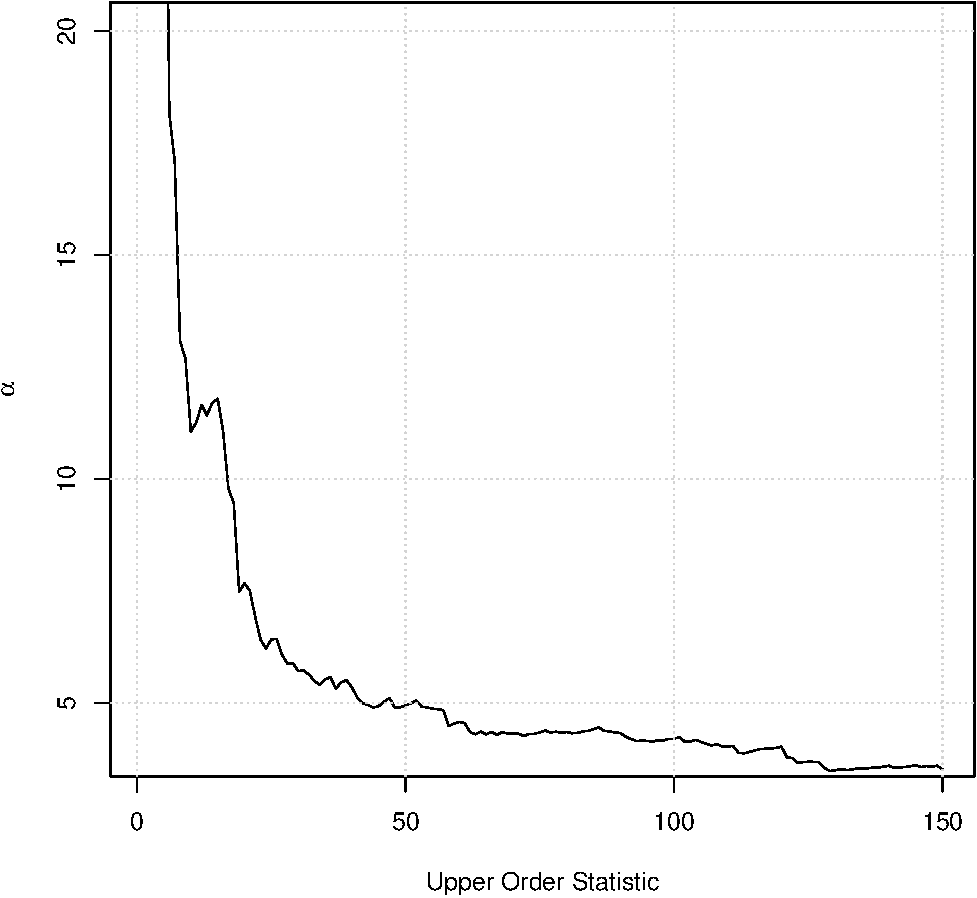
\includegraphics[scale=0.4]{SP500_var_HillPlot.pdf}
%%     \caption{S\&P 500 $\sigma_t^2$ Hill Plot}
%%     \label{fig:SP500_var_HillPlot}
%%   \end{figure}

%% \item GARCH(2, 1)
%%   When fitted to a GARCH(2, 1) process, the S\&P 500 return series has the following model
%%   \[
%%   \sigma_t^2 = 0.088 R_{t-1}^2 + 0.097 R_{t-2}^2 + 0.654 \sigma_{t-1}^2 + 9.2 \times 10^{-6}
%%   \]
%%   \begin{table}[htb!]
%%     \centering
%%     \begin{tabular}{c|c|c|c}
%%       $\alpha$ & $\Lambda(\alpha)$ & abs. err. & rel. err. \\
%%       \hline
%%       0.1000 & -0.0167 & 0.0026 & 0.1550\\
%%       0.2000 & -0.0285 & 0.0051 & 0.1780\\
%%       0.3000 & -0.0353 & 0.0074 & 0.2096\\
%%       0.4000 & -0.0367 & 0.0094 & 0.2566\\
%%       0.5000 & -0.0321 & 0.0120 & 0.3728\\
%%       0.6000 & -0.0221 & 0.0140 & 0.6365\\
%%       0.7000 & -0.0045 & 0.0158 & 3.5121\\
%%       0.8000 &  0.0190 & 0.0195 & 1.0261\\
%%       0.9000 &  0.0500 & 0.0210 & 0.4209\\
%%       1.0000 &  0.0877 & 0.0241 & 0.2747\\
%%     \end{tabular}
%%     \caption{$\Lambda(\alpha)$ of S\&P 500 as GARCH(2,1)}
%%     \label{tab:DAX_garch21_Lambda}
%%   \end{table}
%%   The tail index is estimated at 0.7230.
%% \end{itemize}

%% \subsection{DAX}
%% \begin{itemize}
%% \item GARCH(1, 1)
%%   When modeled as a GARCH(1, 1) process, the DAX return series
%%   has the coefficients as shown in the following equation
%%   \[
%%   \sigma_t^2 = 0.06 R_{t-1}^2 + 0.92 \sigma_{t-1}^2 + 3.1 \times 10^{-6}
%%   \]
%%   \begin{table}[htb!]
%%     \centering
%%     \begin{tabular}{r|r|r|r||r|r|r|r}
%%       $\alpha$ & $\Lambda(\alpha)$ & abs. err. & rel. err. & $\alpha$
%%       & $\Lambda(\alpha)$ & abs. err. & rel. err \\
%%       \hline
%%       0.1000 & -0.0030 & 0.0034 & 1.1195 & 3.6000 & -0.0590 & 0.0554 & 0.9399 \\
%%       0.2000 & -0.0059 & 0.0065 & 1.0900 & 3.7000 & -0.0588 & 0.0543 & 0.9246 \\
%%       0.3000 & -0.0088 & 0.0091 & 1.0396 & 3.8000 & -0.0585 & 0.0557 & 0.9518 \\
%%       0.4000 & -0.0116 & 0.0124 & 1.0668 & 3.9000 & -0.0584 & 0.0570 & 0.9758 \\
%%       0.5000 & -0.0143 & 0.0142 & 0.9911 & 4.0000 & -0.0581 & 0.0583 & 1.0038 \\
%%       0.6000 & -0.0169 & 0.0169 & 1.0009 & 4.1000 & -0.0572 & 0.0584 & 1.0205 \\
%%       0.7000 & -0.0195 & 0.0189 & 0.9701 & 4.2000 & -0.0563 & 0.0600 & 1.0666 \\
%%       0.8000 & -0.0220 & 0.0205 & 0.9315 & 4.3000 & -0.0558 & 0.0569 & 1.0206 \\
%%       0.9000 & -0.0245 & 0.0225 & 0.9199 & 4.4000 & -0.0549 & 0.0591 & 1.0769 \\
%%       1.0000 & -0.0269 & 0.0246 & 0.9155 & 4.5000 & -0.0538 & 0.0618 & 1.1489 \\
%%       1.1000 & -0.0292 & 0.0261 & 0.8921 & 4.6000 & -0.0528 & 0.0623 & 1.1802 \\
%%       1.2000 & -0.0314 & 0.0281 & 0.8969 & 4.7000 & -0.0502 & 0.0627 & 1.2503 \\
%%       1.3000 & -0.0334 & 0.0294 & 0.8820 & 4.8000 & -0.0491 & 0.0637 & 1.2973 \\
%%       1.4000 & -0.0357 & 0.0314 & 0.8802 & 4.9000 & -0.0477 & 0.0630 & 1.3204 \\
%%       1.5000 & -0.0376 & 0.0324 & 0.8616 & 5.0000 & -0.0452 & 0.0645 & 1.4261 \\
%%       1.6000 & -0.0395 & 0.0344 & 0.8712 & 5.1000 & -0.0429 & 0.0675 & 1.5728 \\
%%       1.7000 & -0.0414 & 0.0361 & 0.8730 & 5.2000 & -0.0418 & 0.0657 & 1.5713 \\
%%       1.8000 & -0.0431 & 0.0369 & 0.8542 & 5.3000 & -0.0387 & 0.0640 & 1.6561 \\
%%       1.9000 & -0.0447 & 0.0370 & 0.8270 & 5.4000 & -0.0362 & 0.0699 & 1.9270 \\
%%       2.0000 & -0.0467 & 0.0390 & 0.8340 & 5.5000 & -0.0346 & 0.0695 & 2.0086 \\
%%       2.1000 & -0.0479 & 0.0392 & 0.8184 & 5.6000 & -0.0320 & 0.0687 & 2.1497 \\
%%       2.2000 & -0.0492 & 0.0417 & 0.8477 & 5.7000 & -0.0283 & 0.0704 & 2.4875 \\
%%       2.3000 & -0.0506 & 0.0429 & 0.8482 & 5.8000 & -0.0242 & 0.0692 & 2.8582 \\
%%       2.4000 & -0.0519 & 0.0436 & 0.8393 & 5.9000 & -0.0209 & 0.0694 & 3.3116 \\
%%       2.5000 & -0.0527 & 0.0446 & 0.8450 & 6.0000 & -0.0177 & 0.0709 & 3.9943 \\
%%       2.6000 & -0.0541 & 0.0462 & 0.8540 & 6.1000 & -0.0138 & 0.0704 & 5.1077 \\
%%       2.7000 & -0.0551 & 0.0465 & 0.8446 & 6.2000 & -0.0086 & 0.0702 & 8.1557 \\
%%       2.8000 & -0.0559 & 0.0475 & 0.8483 & 6.3000 & -0.0044 & 0.0739 & 16.8818 \\
%%       2.9000 & -0.0565 & 0.0482 & 0.8522 & 6.4000 & -0.0002 & 0.0718 & 288.3521 \\
%%       3.0000 & -0.0573 & 0.0497 & 0.8677 & 6.5000 &  0.0043 & 0.0722 & 16.9721 \\
%%       3.1000 & -0.0579 & 0.0507 & 0.8756 & 6.6000 &  0.0090 & 0.0762 & 8.4493 \\
%%       3.2000 & -0.0584 & 0.0511 & 0.8755 & 6.7000 &  0.0142 & 0.0789 & 5.5445 \\
%%       3.3000 & -0.0588 & 0.0515 & 0.8766 & 6.8000 &  0.0209 & 0.0769 & 3.6821 \\
%%       3.4000 & -0.0592 & 0.0533 & 0.9002 & 6.9000 &  0.0238 & 0.0789 & 3.3101 \\
%%       3.5000 & -0.0591 & 0.0529 & 0.8953 & 7.0000 &  0.0324 & 0.0772 & 2.3804 \\
%%     \end{tabular}
%%     \caption{$\Lambda(\alpha)$ of DAX as GARCH(1, 1)}
%%     \label{tab:DAX_garch11_Lambda}
%%   \end{table}
%%   The tail index of the stationary distribution of $\sigma_t^2$ is
%%   estimated at 6.4269. The Hill estimator of this
%%   sequence is computed at 6.6020, as the Hill plot in figure
%%   \ref{fig:DAX_var_HillPlot} suggests.
%%   \begin{figure}[htb!]
%%     \centering
%%     \includegraphics[scale=0.4]{DAX_var_HillPlot.pdf}    
%%     \caption{DAX $\sigma_t^2$ Hill Plot}
%%     \label{fig:DAX_var_HillPlot}
%%   \end{figure}

%% \item GARCH(2, 1)
%%   When fitted to a GARCH(2, 1) process, the DAX return series has the following model
%%   \[
%%   \sigma_t^2 = 0.027 R_{t-1}^2 + 0.042 R_{t-2}^2 + 0.897 \sigma_{t-1}^2 + 4.0 \times 10^{-6}
%%   \]
%%   \begin{table}[htb!]
%%     \centering
%%     \begin{tabular}{c|c|c|c}
%%       $\alpha$ & $\Lambda(\alpha)$ & abs. err. & rel. err. \\
%%       \hline
%%       0.1000 & -0.0017 & 0.0026 & 1.5402 \\
%%       0.2000 &  0.0009 & 0.0053 & 6.1829 \\
%%       0.3000 &  0.0077 & 0.0075 & 0.9712 \\
%%       0.4000 &  0.0192 & 0.0096 & 0.4975 \\
%%       0.5000 &  0.0355 & 0.0121 & 0.3411 \\
%%     \end{tabular}
%%     \caption{$\Lambda(\alpha)$ of DAX as GARCH(2,1)}
%%     \label{tab:DAX_garch21_Lambda}
%%   \end{table}
%%   The tail index is estimated at 0.1801.
%% \end{itemize}

% \section{Examples}
% \subsection{GARCH(2, 1)}
% Here we consider the GARCH(2, 1) model described by
% \begin{eqnarray*}
%   \begin{pmatrix}
%     \sigma_{t+1}^2 \\
%     R_t^2 \\
%   \end{pmatrix}
%   =
%   \begin{pmatrix}
%     \alpha_1 z_t^2 + \beta_1 & \alpha_2 \\
%     z_t^2 & 0 \\
%   \end{pmatrix}
%   \begin{pmatrix}
%     \sigma_t^2 \\
%     R_{t-1}^2 \\
%   \end{pmatrix}
% \end{eqnarray*}

% We show that the Markov chain $(\sigma_{t+1}^2, R_t^2)$ satisfies a
% minorization condition for a set $C = [a, b] \times [c, d]$ where
% $a,b,c,d > 0$, and $\forall (x_0, y_0) \in C$
% \begin{eqnarray}
%   && P[(x_0, y_0), I_1 \times I_2] \nonumber \\
%   &=& \P \left[
%       (\sigma_{t+1}^2, R_t^2) \in I_1 \times I_2 |
%       (\sigma_{t}^2, R_{t-1}^2) = (x_0, y_0)
%       \right] \nonumber \\
%   &\geq& \delta' \I_{C}(x_0, y_0) \nu(I_1 \times I_2) \label{eq:Minor}
% \end{eqnarray}
% where $\delta'$ is a constant and $\nu(\cdot)$ is a measure satsifying
% $\nu(C) = 1$.
% \begin{proof}
%   First observe
%   \begin{eqnarray*}
%     && P[(x_0, y_0), I_1 \times I_2] \\
%     &=& \int_{I_1} \int_{I_2}
%         \delta \left[
%         \alpha_1 x + \beta_1 x_0 + \alpha_2 y_0 - y
%         \right]
%         f_{x_0 Z^2}(x) dx dy
%   \end{eqnarray*}
%   where $\delta(\cdot)$ is the Dirac-$\delta$ function.
%   Simplifying the above equation gives
%   \begin{eqnarray*}
%     && P[(x_0, y_0), I_1 \times I_2] \\
%     &=& \int_{I_1/x_0} \I_{I_2}(\alpha_1 x_0 z^2 + \beta_1 x_0 +
%         \alpha_2 y_0) f_Z^2 (z^2) dz^2
%   \end{eqnarray*}
%   Define mapping
%   \begin{equation*}
%     g(s, x, y): s \rightarrow {s \over \alpha_1 x}
%     - \left(
%       {\alpha_2 \over \alpha_1} {y \over x} + {\beta_1 \over \alpha_1}
%     \right)
%   \end{equation*}
%   for $s \in (\alpha_2 y + \beta_1 x, \infty)$ and $x, y
%   \in \mathbb R_+$. Then we may write
%   \begin{eqnarray*}
%     && P[(x_0, y_0), I_1 \times I_2] \\
%     &=& \int_{I_1 / x_0 \cap g(I_2, x_0, y_0)} f_{Z^2}(z^2) dz^2
%   \end{eqnarray*}
%   Define a subset $h(I_2)$ of $I_2$:
%   \[
%   h(I_2) = I_2 \cap (\alpha_2 d, \infty)
%   \]
%   Note if $h(I_2) \neq \emptyset$ then $\forall s \in h(I_2)$ and $\forall
%   y \in [c, d]$
%   \begin{equation}
%     \label{eq:der_g}
%     \pd{g(s, x, y)}{x} < 0    
%   \end{equation}
%   So we have
%   \begin{eqnarray*}
%     && P[(x_0, y_0), I_1 \times I_2] \\
%     &\geq& \int_{I_1/x_0 \cap g(h(I_2), x_0, y_0)} f_{Z^2}(z^2) dz^2
%   \end{eqnarray*}
%   Since $Z^2 \sim \chi^2(1)$, $f_{Z^2}(z^2)$ is monotonically
%   decreasing. Meanwhile, $\L g(h(I_2), x_0, y_0)$, the Lebesgue measure
%   of $g(h(I_2), x_0, y_0)$ is the smallest when $x_0$ is the
%   largest possible, i.e. $b$. Furthermore, \eqref{eq:der_g} shows
%   \[
%   \arg \max_{x \in [a, b]} g(s, x, y) = a
%   \]
%   Hence
%   \begin{eqnarray*}
%     && \int_{I_1/x_0 \cap g(h(I_2), x_0, y_0)} f_{Z^2}(z^2) dz^2 \\
%     &\geq& \int_{J(I_1, I_2)} f_{Z^2}(z^2) dz^2           
%   \end{eqnarray*}
%   where $J(I_1, I_2) := \emptyset$ if $I_1 = \emptyset$ or $h(I_2) =
%   \emptyset$; otherwise
%   \begin{eqnarray*}
%   && J(I_1, I_2) \\
%   &:=& [\max I_1/a - \L I_1/b, \max I_1/a]
%       \cap \\
%   && [g(\max h(I_2), a, c) - \L h(I_2) /\alpha_1 b, g(\max h(I_2), a, c)]
%   \end{eqnarray*}
%   Clearly
%   \begin{eqnarray*}
%     && \int_{J(I_1, I_2)} f_{Z^2}(z^2) dz^2               \\
%     &\geq& \int_{J(I_1, I_2) \cap J([a, b], [c, d])} f_{Z^2}(z^2)
%            dz^2 \\
%     &\geq& f_{Z^2}(\max J([a, b], [c, d])) \L J([a, b], [c, d])
%            {
%            \L \left(
%            J(I_1, I_2) \cap J([a, b], [c, d])
%            \right)
%            \over
%            \L J([a, b], [c, d])
%            }
%   \end{eqnarray*}
%   Thus \eqref{eq:Minor} is satisfied with
%   \begin{eqnarray}
%     \delta'
%     &=&
%     f_{Z^2}(\max J([a, b], [c, d])) \L J([a, b], [c, d]) \label{eq:regen_prob}\\
%     \nu(I_1 \times I_2)
%     &=& {
%       \L \left(
%         J(I_1, I_2) \cap J([a, b], [c, d])
%       \right)
%       \over
%       \L J([a, b], [c, d])
%     } \nonumber
%   \end{eqnarray}
% \end{proof}
% From \eqref{eq:regen_prob} it immediately follows that $\delta'$ is
% maximized by $J([a, b], [c ,d])$ satisfying
% \begin{eqnarray}
%   x_\M &=& {
%     1 + x_\m + \sqrt{x_\m^2 + 6 x_\m + 1}
%     \over
%     2
%   } \label{eq:maximizing_cond}
% \end{eqnarray}
% where 
% \begin{eqnarray*}
%   x_\M &=& \max J([a, b], [c ,d]) \\
%   x_\m &=& \min J([a, b], [c ,d])
% \end{eqnarray*}
% Since
% \[
% J([a. b], [c, d]) =
% \left[
%   {b \over a} + {a \over b} - 1, {b \over a}
% \right] \bigcap \left[
%   {d - \alpha_2 c \over \alpha_1 a} - {\beta_1 \over \alpha_1} -
%   {d \over \alpha_1 b} + {\alpha_2 d \wedge c \over \alpha_1 b},
%   {d - \alpha_2 c \over \alpha_1 a} - {\beta_1 \over \alpha_1}  
% \right]
% \]
% One way to choose $a, b, c, d$ so as to maximize $\delta'$ is to first
% choose $c = 0$ and then choose $a, b$ so that
% \eqref{eq:maximizing_cond} is satisfied by $b/a + a/b - 1$ and $b/a$
% as $x_\m$ and $x_\M$ respectively. Finally choose
% \[
%   \alpha_1 b + \beta_1 a
%   \leq
%   d
%   \leq
%   \alpha_1 {
%     a^2 - ab + b^2
%     \over
%     b - a
%   } +
%   \beta_1 {
%     ab \over b - a
%   }
% \]
% It is easily verified that the above interval for $d$ has length
% ${a^2 \over b - a} (\alpha_1 + \beta_1) > 0$. With such choices
% \[
% J([a. b], [c, d]) =
% \left[
%   {b \over a} + {a \over b} - 1, {b \over a}
% \right]
% \]
% If $b/a$ is chosen to be the root of
% \[
% x^4 - 9x^2 + 6x - 6 = 0
% \]
% in the interval $(1, \infty)$, $b/a + a/b - 1$ and $b/a$ satisfy
% \eqref{eq:maximizing_cond}. Figure \ref{fig:A} shows the function
% $f(x) = x^4 - 9x^2 + 6x - 6$ in $(1, \infty)$.
% \begin{figure}[htb!]
%   \centering
%   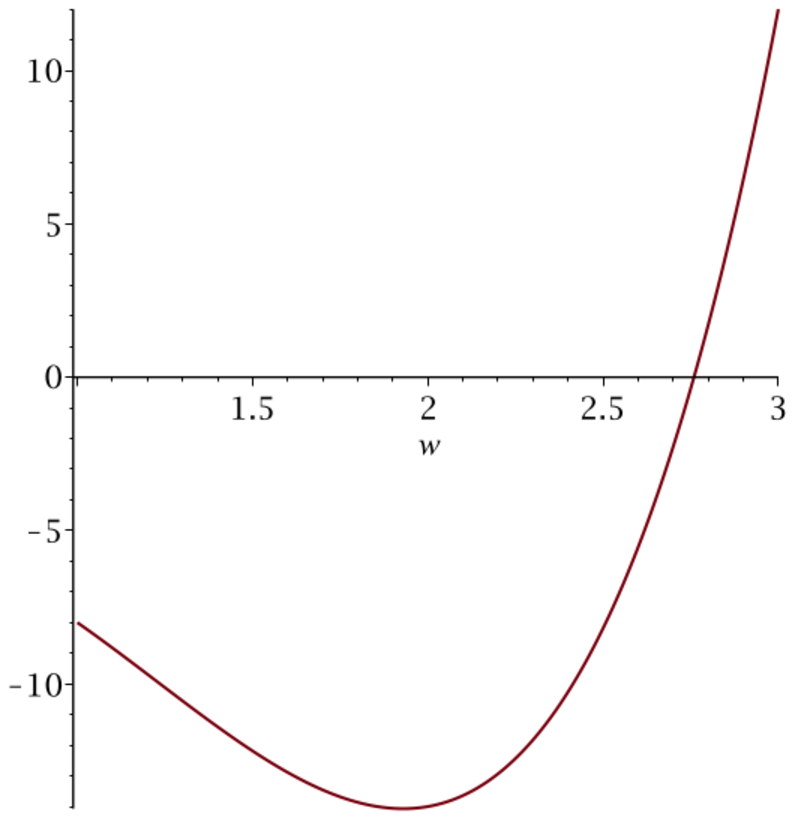
\includegraphics[scale=0.4]{argmax_b_over_a.pdf}
%   \caption{Graph of $f(x) = x^4 - 9x^2 + 6x - 6$}
%   \label{fig:A}
% \end{figure}
\bibliographystyle{unsrt}
\bibliography{../../thesis/econophysics}
\end{document}
